

\title{A Framework for Collecting, Extracting and Managing Event Identity Information from Textual Content in Social Media}
\author{
        Debanjan Mahata \\
                Department of Information Science\\
        University of Arkansas at Little Rock\\
        Little Rock, Arkansas, USA
}

\date{}
\documentclass[11pt, oneside]{Thesis} % The default font size and one-sided printing (no margin offsets)

\graphicspath{{Pictures/}} % Specifies the directory where pictures are stored

\usepackage[square, numbers, comma, sort&compress]{natbib} % Use the natbib reference package - read up on this to edit the reference style; if you want text (e.g. Smith et al., 2012) for the in-text references (instead of numbers), remove 'numbers' 
\usepackage{caption}
\usepackage{subcaption}
\usepackage{multirow}
\usepackage{booktabs}
%\usepackage{hyperref}
\usepackage{footnote}
\usepackage{amsmath}
\usepackage{algorithm2e}
\usepackage{amssymb}
\usepackage{titlesec}
\usepackage{graphicx}

\begin{document}
\maketitle

Social media has brought a paradigm shift in the way people communicate with each other. It has gone from being just a medium to a global medium of communication between people. Different types of social media platforms provide multiple venues to people for sharing first-hand experiences and exchange information about real-life events. It has become an indispensable source for disseminating news and real-time information about current events, using websites like Twitter, Facebook, Instagram, Flickr, Youtube, Vine, etc, that allow users to post short textual messages accompanied with images and videos. At the same time users also share their detailed citizen journalistic experiences in the form of diaries through different blogging platforms like Blogger, Wordpress, Medium, etc. Studies have shown the importance of different social media platforms as a news circulation service \cite{phelan2009using}, and a source for gauging public interest and opinions \cite{o2010tweets,singh2010clustering,singh2010mining,agarwal2012online}. It's efficacy as a real-time citizen-journalistic source of information has been recently harnessed in detection, extraction and analysis of real-life events \cite{sakaki2013tweet,popescu2011extracting,purohit2013twitris}. The activities of users producing content in social media has also been studied for gaining deep insights about how they group together to form communities around topics related to real-life events \cite{agarwal2013grouping,agarwal2014time,sen2012identifying}, and lead to collective action \cite{agarwal2014online,agarwal2012raising}.

With the popularity of social media there has been proliferation of unstructured textual content about different real-life events, in the Internet.
The information gained by identifying and tracking social media content expressing live reporting of an event, recent updates related to the event, insightful opinion about the different named entities (people, place, organization, etc) directly or indirectly involved with the event, summarization of content, among others, could prove to be extremely valuable for monitoring and gaining deeper actionable insights. There are tremendous applications in the areas of real-life event analysis, event management, opinion mining, reference tracking, online targeted marketing, recommendation engines, cyber security, enterprise data integration, among others. Thus, there is a need of a generic framework that has the following capabilities:
\begin{itemize}
\item can collect different types of textual content produced in social media related to an event
\item extract information that acts as an identity of the event used for characterizing it
\item maintain the extracted event identity information persistently for resolving constantly produced new content and discovering important event-specific information. 
\end{itemize}


The problem of collecting and extracting event identity information from social media is very similar to the task of event detection and tracking from newswires \cite{allan1998line,kumaran2004text}. However, in this thesis, we add new components of creating identity structures of an event and managing the tracked information persistently over time. In order to make our task well defined we avoid the task of detecting unidentified events, and instead track a pre-specified set of events. Also, the domain of social media poses additional challenges. News articles most often adhere to grammatical, syntactical and formal structures of writing, that are not common in the realm of social media. The user generated content in social media is most often colloquial, short, noisy and lack proper grammatical structures. This makes it a challenging task for the state-of-the-art natural language processing techniques to extract useful information and perform tasks like entity extraction and parts-of-speech tagging that lies at the core of the previous research on event detection and tracking.

The work presented in this thesis establishes the conceptual design and implementation of a framework capable of collecting, extracting and persistently managing event identity information from user generated textual content shared in social media (shown in Figure 1.1). The approach of the presented work is from the perspective of Entity Identity Information Management (EIIM) \cite{zhou2011entity}, with basic tenets of information quality at its core. Towards this objective, different challenges of mining high quality information from social media text is discussed and a patent pending novel approach to tackle the challenges for identifying event-specific informative content is explained, which lies at the heart of the framework. It further explores the applications of the research and concludes by pointing to different future directions of the work. 


%The thesis introduces the problem of Event Identity Information Management in social media, discusses the prevalent challenges and presents the implementation design of a framework capable of managing persistent identity information of pre-specified set of real-life events. It further explores the applications of the research and concludes by pointing to different future directions of the work. 

\begin{figure}[htbp]
\label{eiim}
  \caption{Event Identity Information Management (EIIM) Life Cycle for user generated textual content in social media}
  \centering
    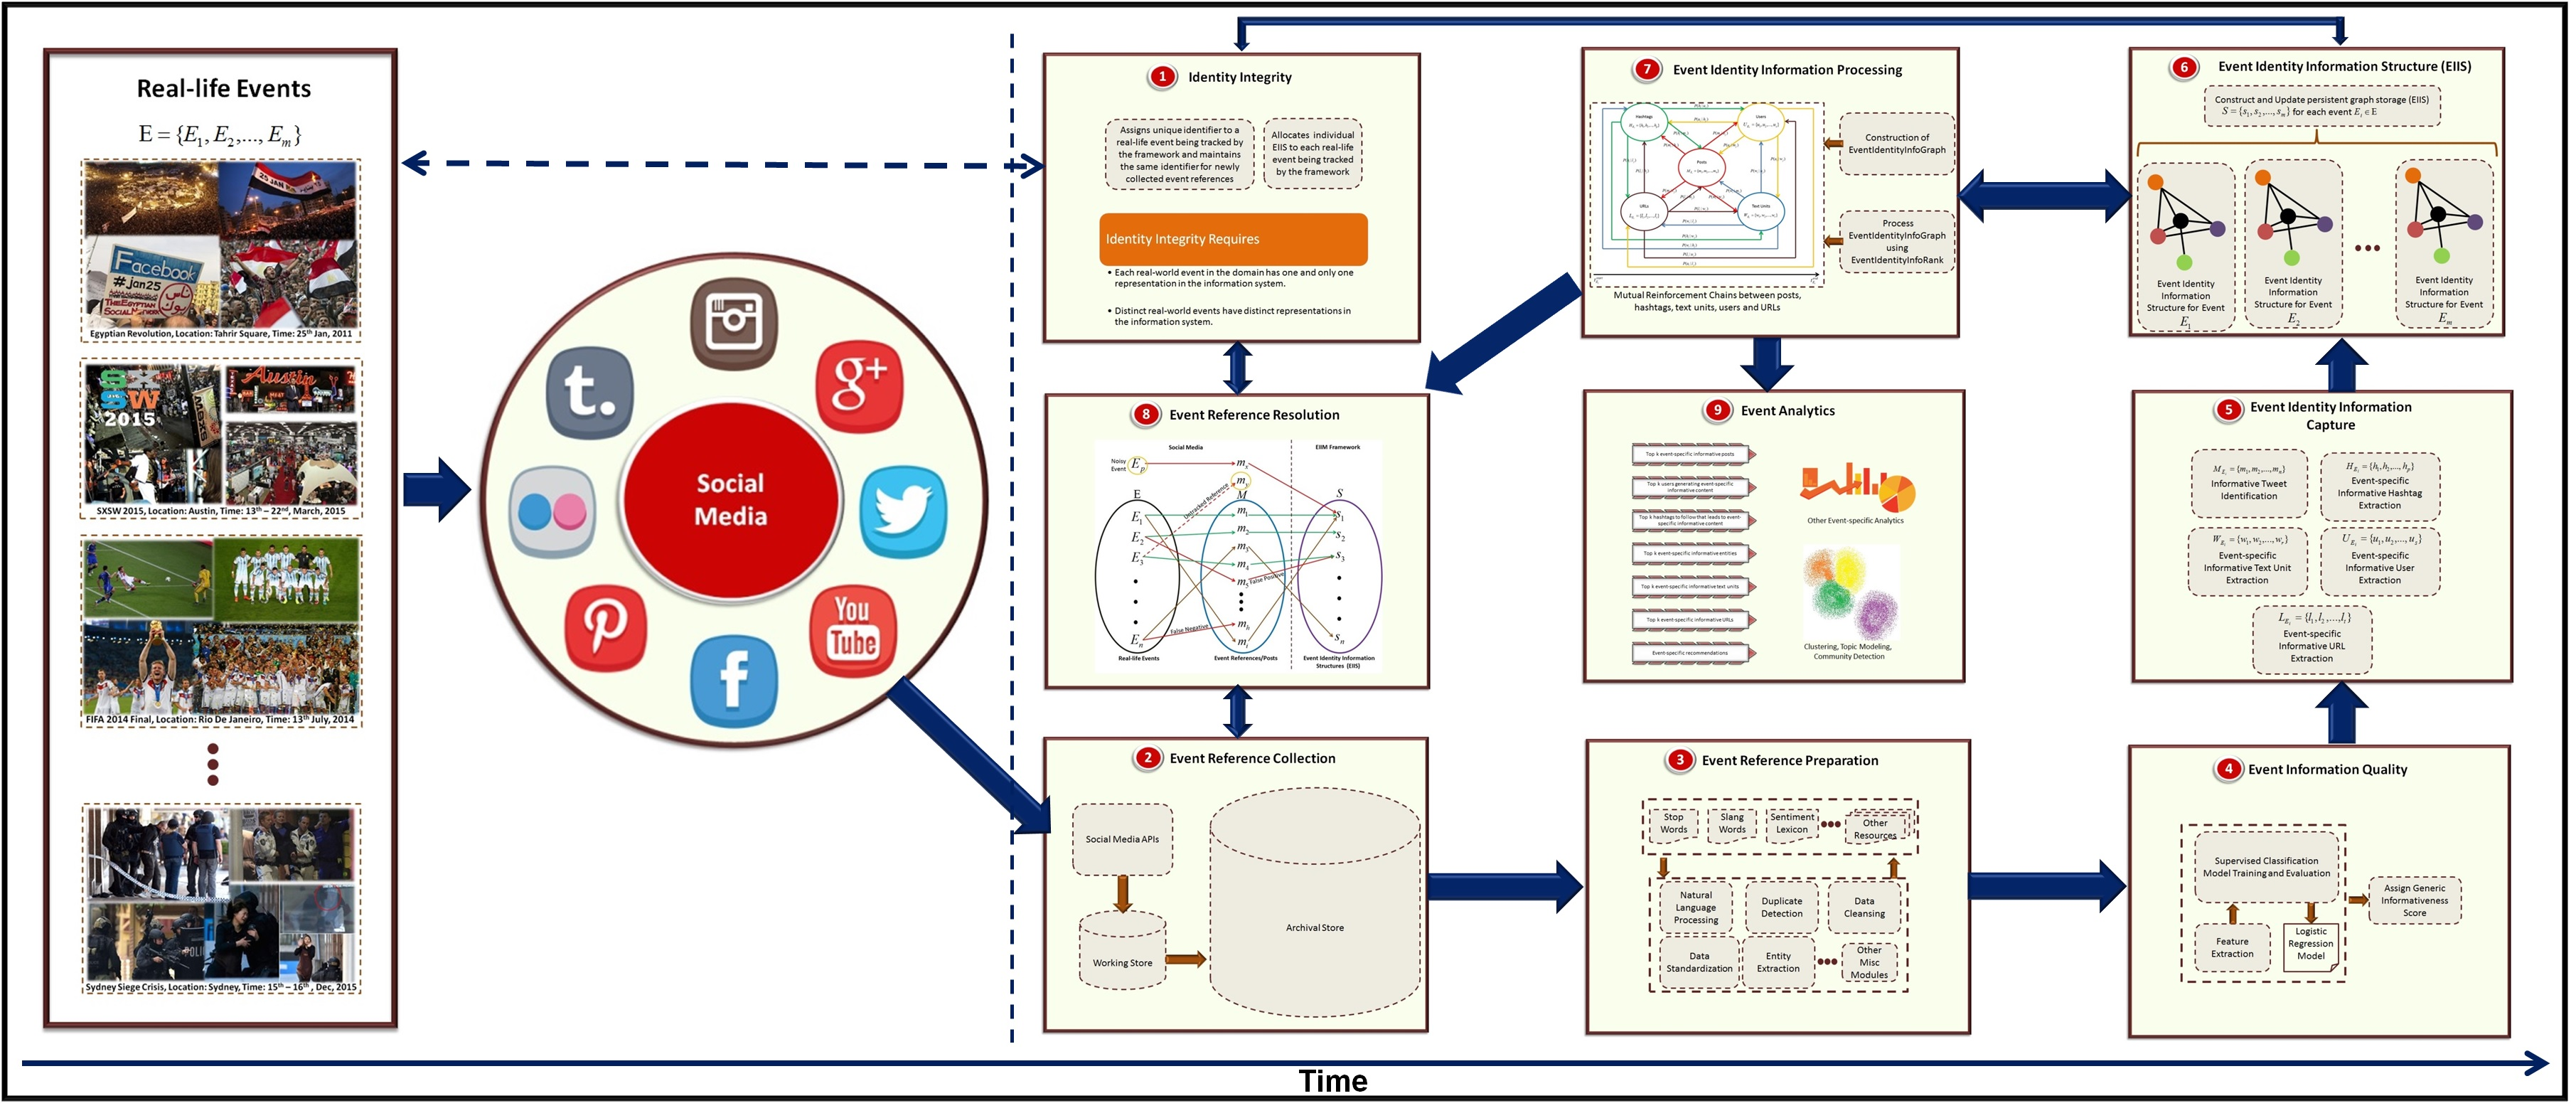
\includegraphics[width=15.5cm,height=7cm]{Figures/EIIM.jpg}
\end{figure}

Some of the main contributions of the work are:

\begin{itemize}
\item Extending the Entity Identity Information Management model  \cite{zhou2011entity} from the closed world domain of Master Data Management (MDM) to the open and unstructured domain of social media.

\item Design and implementation of an \textit{Event Identity Information Management} framework that is capable of tracking and identifying event-specific information from long as well as short user generated textual content in social media. Towards this objective a data processing pipeline named \textit{Event Identity Information Management Life Cycle} is developed (Figure 1.1), which is capable of :
\begin{itemize}
\item collecting event related real-time content generated in social media
\item pre-processing them using natural language processing techniques
\item identifying high quality informative sources of information
\item extracting event-specific information in order to create \textit{Event Identity Information Structures} (EIIS) for persistently storing and characterizing the salient and high quality event related information 
\item identifying event-specific informative content produced in social media
\end{itemize}


\item Implementation of a supervised classifier in the domain of short and informal social media textual content, for segregating high quality informative messages having higher chances of containing event related information from the low quality non-informative ones. 

\item Analysis of informative and non-informative event related content from 3.8 million short textual social media messages.

\item A novel model that leverages mutually reinforcing relationships between blog posts and named entities mentioned in them, and simultaneously ranks blogs as well as the named entities, allowing identification of event-specific content and further analysis of event-specific information.

\item A novel model based on principle of mutual reinforcement that takes into account the semantics of relationships between short textual \textit{social media messages}, \textit{hashtags}, \textit{text units}, \textit{URLs} and \textit{users}, and represent them in a graph structure - \textit{EvenIdentitytInfoGraph}. A scalable graph processing iterative algorithm -\textit{EventIdentityInfoRank}, is implemented for ranking the nodes of the \textit{EventIdentityInfoGraph}. The algorithm is capable of simultaneously ranking \textit{social media messages}, \textit{hashtags}, \textit{text units}, \textit{URLs} and \textit{users} in terms of event-specific informativeness providing deeper insights into the identity of an event.

\item Evaluation of the proposed techniques against popularly used baseline techniques using large scale datasets.

\end{itemize}

Already published work as well as upcoming publications that represents our contributions related to specific topics covered by the broad area of research as presented in this thesis are given below. \\ 

\textbf{\LARGE Related Filed Patent}
\begin{itemize}
\item A System for Collecting, Ranking and Managing Entity Identity Information from Social Media (US 62135258). Inventors: \textbf{Debanjan Mahata} and John R. Talburt, Assignee: The Board Of Trustees Of The University Of Arkansas.
\end{itemize}

\textbf{\LARGE Related Award}
\begin{itemize}
\item \textbf{Debanjan Mahata} and John R. Talburt. \textit{Chatter that Matter : A Framework for Collecting, Extracting, and Managing Event Identity Information from Short Social Media Text}. Student Research and Creative Works Expo, Graduate Competition, University of Arkansas at Little Rock, April, 2015. (Awarded First Place in Engineering and Information Technology).  
\end{itemize}

\textbf{\LARGE Related Publications}
\begin{itemize}
\item \textbf{Debanjan Mahata}, John R. Talburt and Vivek Kumar Singh; \textit{Identifying and Ranking of Event-specific Entity-centric Informative Content from Twitter}. $20^{th}$ International Conference On Applications Of Natural Language To Information Systems (NLDB 2015), Passau, Germany. $17^{th}-19^{th}$ June, 2015.

\item \textbf{Debanjan Mahata} and John R. Talburt; \textit{A Framework for Collecting and Managing Entity Identity Information from Social Media}. $19^{th}$ International Conference on Information Quality, Xi'An, China.

\item \textbf{Debanjan Mahata} and Nitin Agarwal; \textit{Identifying Event-specific Sources from Social Media}. Online Social Media Analysis and Visualization. Lecture Notes in Social Networks, Springer, Kawash, Jalal (Ed). January, 2015.

\item Nitin Agarwal, \textbf{Debanjan Mahata}, and Huan Liu. \textit{Time-and Event-Driven Modeling of Blogger Influence}. Encyclopedia of Social Network Analysis and Mining. Springer New York, 2014. 2154-2165.


\item \textbf{Debanjan Mahata} and Nitin Agarwal. \textit{Learning from the crowd: An Evolutionary Mutual Reinforcement Model for Analyzing Events}. Advances in Social Networks Analysis and Mining (ASONAM), 2013 IEEE/ACM International Conference on. IEEE, 2013.

\item Nitin Agarwal, and \textbf{Debanjan Mahata}. \textit{Grouping the Similar among the Disconnected Bloggers}. Social Media Mining and Social Network Analysis: Emerging Research (2013), 54.

\item \textbf{Debanjan Mahata}, and Nitin Agarwal. \textit{What does everybody know? identifying event-specific sources from social media}. IEEE Fourth International Conference on Computational Aspects of Social Networks (CASoN), 2012.

\item \textbf{Debanjan Mahata} and Nitin Agarwal. \textit{Analyzing Event-specific Socio-Technical Behaviors Through the Lens of Social Media}. The International Sunbelt Social Network Conference (Sunbelt XXXII) organized by the International Network for Social Network Analysis (INSNA), March 12-18, 2012, Redondo Beach, California.

\item Vivek Kumar Singh, \textbf{Debanjan Mahata}, and Rakesh Adhikari. \textit{Mining the blogosphere from a socio-political perspective}. IEEE International Conference on Computer Information Systems and Industrial Management Applications (CISIM), 2010.

\item Vivek Kumar Singh, Rakesh Adhikari, and \textbf{Debanjan Mahata}. \textit{A clustering and opinion mining approach to socio-political analysis of the blogosphere}. IEEE International Conference on Computational Intelligence and Computing Research (ICCIC), 2010.

\end{itemize}

\textbf{\LARGE Related Submitted Publications}

\begin{itemize}
\item \textbf{Debanjan Mahata}, John R. Talburt, Vivek Kumar Singh and Rajesh Piryani; \textit{Chatter that Matter: A Framework for Identifying and Ranking Event-specific Informative Tweets}. $18^{th}$ International Conference on Text, Speech and Dialogue, Plzen, Czech Republic (Notification Due: May 10, 2015)

\item \textbf{Debanjan Mahata}, John R. Talburt and Vivek Kumar Singh; \textit{A Framework for Collecting, Extracting and Managing Event Identity Information from Twitter}. $20^{th}$ International Conference on Information Quality, M.I.T, Boston (Notification Due: April 30, 2015)

\item \textbf{Debanjan Mahata}, John R. Talburt and Vivek Kumar Singh; \textit{From Chirps to Whistles : Discovering Event-specific Informative Content from Twitter}. Proceedings of the $7^{th}$ Annual ACM Web Science Conference. ACM, 2015, Oxford, England (Notification Due: April 30, 2015)

\end{itemize}
  
%\label{Bibliography}

%\lhead{\emph{Bibliography}} % Change the page header to say "Bibliography"

\bibliographystyle{abbrv} % Use the "unsrtnat" BibTeX style for formatting the Bibliography

\bibliography{Bibliography} % The references (bibliography) information are stored in the file named "Bibliography.bib"


\end{document}
This is never printed